\documentclass[12pt,twoside]{article}   
\usepackage{light, graphicx}

\newcommand{\lr}{l_{right}}
\renewcommand{\ll}{l_{left}}

%\hidesolutions
\showsolutions

%requirements:
% 2 induction  problems
% 2 new candidate problems
% topics: section 5.4 - 5.7 6.1-6.2
% namely:
%walks and paths  (candidate problem on multiplication)
%connectivity and connectedness - builup error
%cycles - die hard cycle (also bipartite, coloring)
%trees - n - 1 edges for n vertices
%dags and digraphs -

%tournaments

%%%%%%%%%%%%%%%%%%%%%%%%%%%5
\begin{document}
\problemset{5}{October 5, 2010}{Tuesday, October 12 at 7pm}
Readings: Section 5.4 to 5.7 and 6.1-6.2.

\begin{problem}{20}
Recall that a tree is a connected acyclic graph.  In particular, a single vertex is a tree.  We define a \emph{Splitting Binary Tree}, or \emph{SBTree} for short, as either the lone vertex, or a tree with the following properties:

\begin{enumerate}
\item  exactly one node of degree 2 (called the root).
\item  every other node is of degree 3 or 1 (called internal nodes and leaves, respectively).
\end{enumerate}

For the case of one single vertex (see above), that vertex is considered to be a leaf.  It is easier to understand the definition visually, so an example is shown in Figure 1. An example of a tree which is not an SBTree is shown in Figure 2.

\begin{figure}[p]
\label{split}
\centerline{\includegraphics[width = 3.00in]{splittingTree}}
\caption{Splitting Binary Tree: Node A is the root, B and E are internal nodes, and C, D,  F, and G are leaves.  Notice how all internal nodes have degree $3$.}
\end{figure}


\begin{figure}[p]
\label{binary}
\centerline{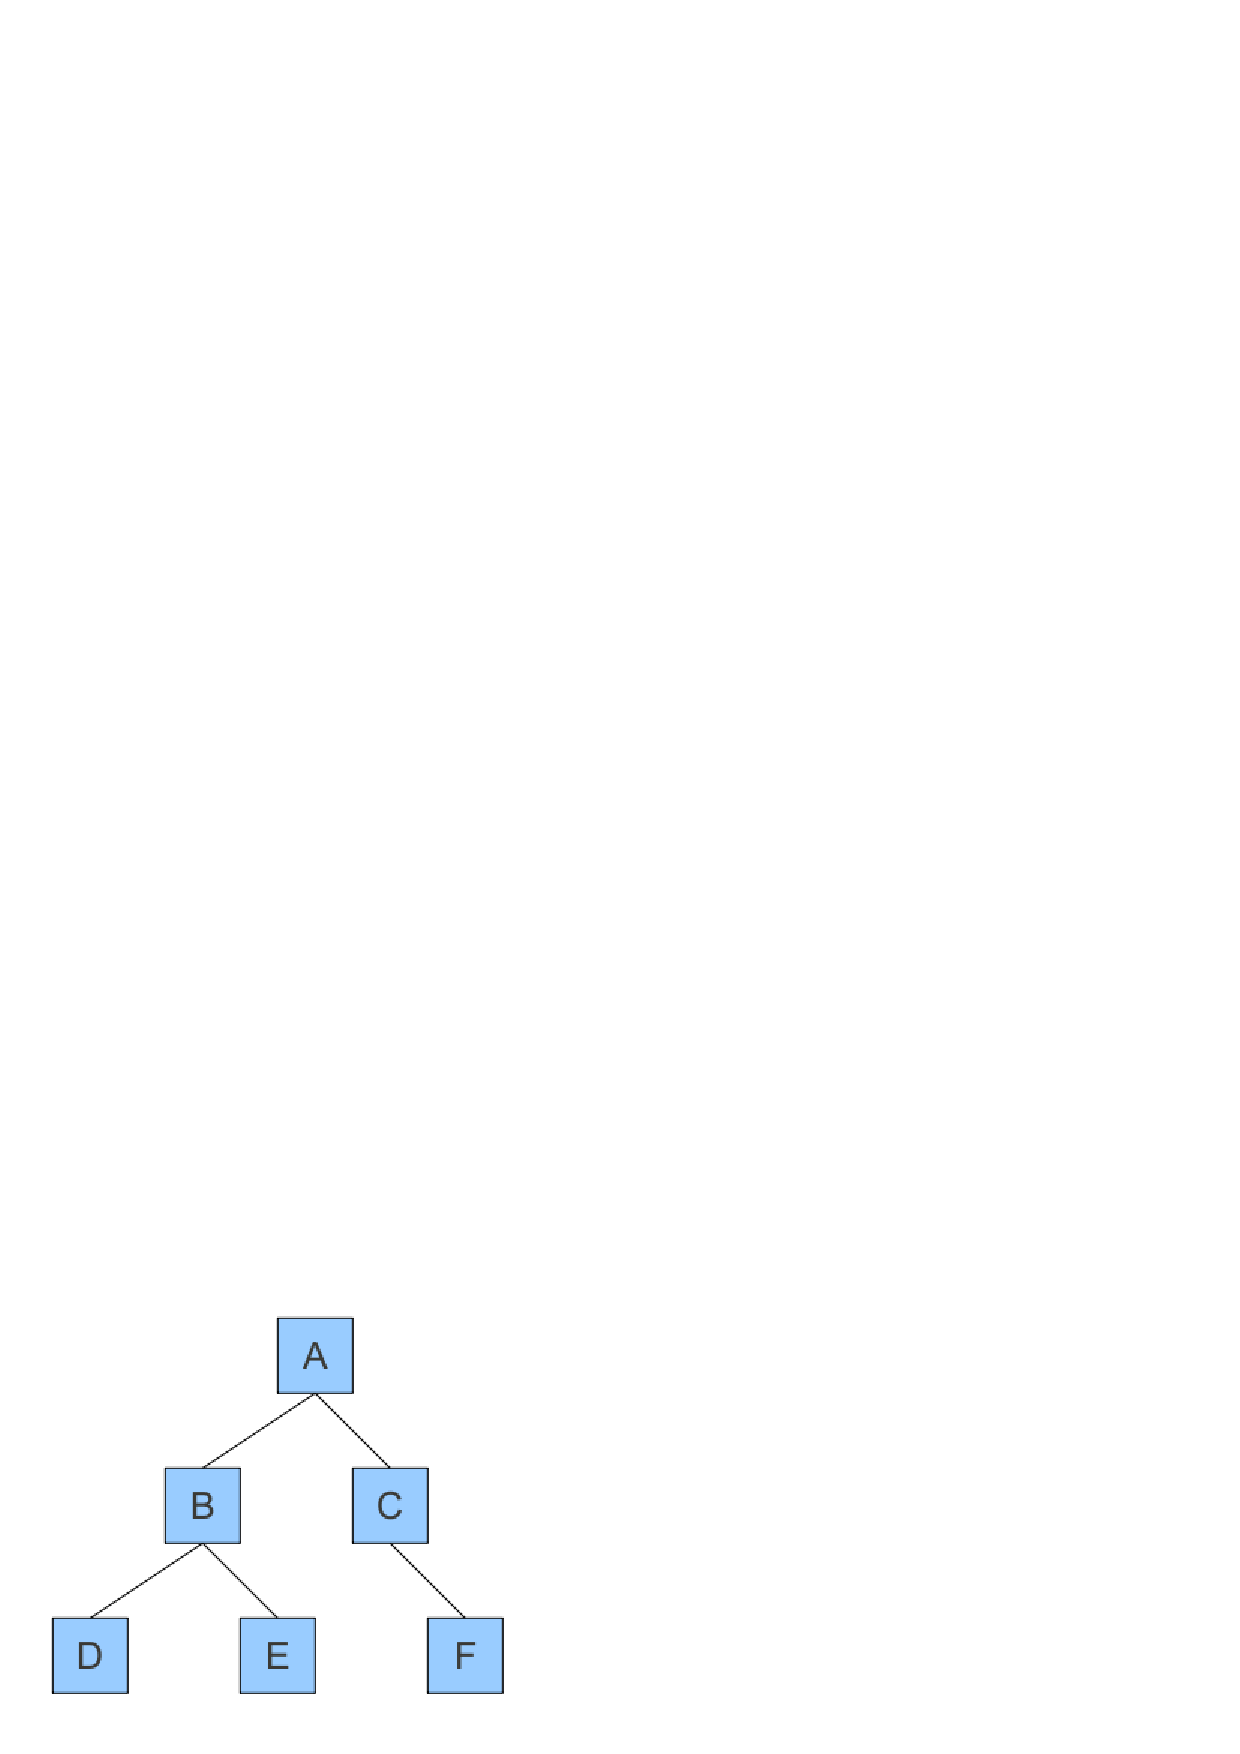
\includegraphics[width = 3.00in]{binaryTree}}
\caption{This is an example of a tree which is NOT a Splitting Binary Tree.  Notice how both A and C have degree $2$, when a BSTree can only have one such node.}
\end{figure}

\begin{problemparts}

\ppart {10} Show if an SBTree has more than one vertex, then the induced subgraph obtained by removing the unique root consists of two disconnected SBTrees. You may assume that by removing the root you obtain two separate connected componenents, so all you need to prove is that those two components are SBTrees.

\solution{ 
Consider one of the two connected components. We must show it is:

\begin{enumerate}
\item Connected: we get this for free because this is a connected component.
\item Acyclic: suppose there is a cycle in our component. Since this component is a subgraph of the original SBTree, then the original SBTree would have had a cycle.
\item SBTrees: by showing it is connected and acyclic, we have checked it is a tree. Now it remains to show it is also an SBTree. We have two cases to consider. Perhaps the node connected to the root (in our connected component) had degree 1 originally, in which case the full connected component is a lone vertex, and hence an SBTree.  Otherwise, the node was of degree 3 originally, so it is now a degree 2 node. Any other remaining node in the connected component would have its degree intact, so it must be of degree 3 or 1. Hence the connected component is an SBTree.
\end{enumerate}
}

\ppart {10} Prove that two SBTrees with the same number of leaves must also have the same total number of nodes. \emph{Hint: As a conjecture, guess an expression for the total number of nodes in terms of the number of leaves $N\left(l\right)$.  Then use induction to prove that it holds for all trees with the same \( l \)}

\solution{ 
You can deduce a formula by experimentation. Our guess is  \( N\left(l\right) = 2l - 1 \). 

\begin{proof}
We will now verify this formula by strong induction on $l$, the number of leaves. 

\begin{enumerate}
\item  Base case:
  If $l = 1$ Then we have one leaf, hence this is the sinlge vertex SBTree. So the total number of nodes is \( 1 \) which agrees with our formula: \( 2\cdot 1 - 1 \).

\item Induction step:

  Assume that for all \(1 \leq l \leq k\), an SBTree with \( l \) leaves in it has \( 2l - 1 \) nodes in total, regardless of its particular structure. We wish to prove that every SBTree of size \( k + 1 \) has \(2 \left(k + 1 \right) - 1\) nodes in total. Consider a generic SBTree with \(k + 1 \) leaves. We assume \(k\) is greater than or equal to 1, so our graph has two subgraphs connected to a root. From the first part we know each is an SBTree. 

  We cannot assume anything about their structure, but we know  if denote by \( \ll \) the  number of leaves in the left child, and by \( \lr \) the number of leaves in the right side then we must have \( k + 1 = \ll + \lr \). And also, \( 0 < \ll\mbox{, } \lr < k + 1 \). Hence, by our induction hypothesis, the number of nodes in the left is \( N \left(  \ll \right)  = 2\ll - 1 \) and the number of nodes in the right is \(N \left( \lr \right) = 2\lr - 1\). And the total number of nodes in the tree must be \(N \left(\lr \right) + N(\ll) + 1\), accounting for the root. Substituting, we get \( 2\lr - 1 + 2\ll - 1  + 1 = 2(\lr + \ll) - 1 = 2(k+1) - 1 \), as we wanted to show.
\end{enumerate}

\end{proof}

}
\eparts

\end{problem}


\begin{problem}{20}
%topics: hamiltonian cycles, two coloring - bipartite, induction

In "Die Hard: The Afterlife", the ghosts of Bruce and Sam have been
sent by the evil Simon on another mission to save  midtown
Manhattan. They have been told that there is a bomb on a street
corner that lies in Midtown Manhattan, which Simon defines as
extending from 41st Street to 59th Street and from 3rd Avenue to 9th
Avenue. Additionally, the code that they need to defuse the bomb is
on another street corner. Simon, in a good mood, also tosses them
two carrots:

\begin{itemize}
\item He will have a helicopter initially lower them to the street corner where the bomb is.
\item He promises that the code is placed only on a corner of a numbered
street and a numbered avenue, so they don't have to search Broadway.
\end{itemize}

The map of midtown Manhattan is an example of an $N \times M$
(undirected) grid.  In particular, midtown Manhattan is a $19 \times
7$ grid.

%INSERT FIGURE of 19 by 7 grid

Bruce and Sam need to check all $19 \cdot 7 = 133$ street corners
for the code.  Once they are at a corner, they don't need any
additional time to verify if the code is there.  Once they find the
code and return to the bomb, they can disarm it in 2 minutes (even,
or especially, as the timer ticks down to 0). Also, they can run one
block (in any of the four directions) in exactly 1 minute.
%(even though avenue blocks are longer than
%street blocks in NYC, it takes them the same amount of time for each
%kind).
They are given 135 minutes total in which to find the code and
disarm the bomb, which means that they need to return to the bomb,
code in hand, in 133 minutes.

Sam realizes that the map of NYC is actually a graph, and that they
need to use a cool new 6.042 concept: A {\em Hamiltonian cycle} is a
path that visits each vertex in a graph exactly once and ends at its
starting point (so it is a cycle). A graph is {\em Hamiltonian} if
it has a Hamiltonian cycle.

Hamiltonian graphs are really useful because you can visit each node
and return to the starting point by taking only $n$ steps, where $n$
is the number of nodes -- if a graph is not Hamiltonian, you would
need at least $n+1$ steps to visit each of the $n$ nodes and return
to the starting point.

In general, we don't know how to efficiently determine whether a
general graph is Hamiltonian or not. However, Sam is very excited
because he thinks that he can show that Midtown Manhattan is
Hamiltonian.  If it is, Bruce and Sam can save the day! Will they
make it?

\bparts

\ppart {10} Show that they cannot do it -- that is, more generally,
show that if both $N$ and $M$ are odd, then the $N\times M$
grid is {\em not} Hamiltonian. {\em Hint:
First show that any $N \times M$ 2-dimensional undirected grid is
bipartite.}
\solution{ As per the hint, let us first show that any 2-dimensional grid 
is bipartite. For this, let us exhibit a coloring with 2 colors $\{0,1\}$. 
Indexing 
the vertices of the grid by their $(x,y)$-coordinates, color vertex 
$(i,j)$ with color $rem(i+j, 2)$. It is easy to see that this is a valid 
2-coloring.

Suppose the graph is Hamiltonian.
Now, since $N,M$ are both odd, there are an odd number of vertices in the 
graph. Thus the hamiltonian cycle in this graph is an odd cycle. However, 
since the graph is bipartite, this graph has no odd cycles. This is a 
contradiction: thus our supposition that the graph was Hamiltonian is 
wrong, and we are done.
}

\ppart {10}
Suppose Simon defined Midtown in the more standard way
as extending from 40th Street to 59th Street and from 3rd Avenue to 9th
Avenue (that is suppose Midtown Manhattan was a $20 \times 7$ grid),
and gave them another 7 minutes,
\begin{enumerate}
\item
Show that if either $N$  is  even and $M > 1$ or  $M$ is even and $N > 1$, then the $N\times M$ grid is Hamiltonian.
\solution{Suppose $N$ is even (wlog).  We give a direct proof and an inductive proof.

Direct constructive proof:

Assume the grid is laid out on the plane occupying the integer points 
between $(0,0)$ and $(N-1, M-1)$.

We will give the hamiltonian path explicitly by specifying the $k$'th 
vertex visited for each $k$ from $0$ to $NM$. Let $q = \lfloor 
\frac{k}{M-1} \rfloor$ and let $r = rem(k, M-1)$.

On step $k$:
\begin{itemize}
\item if $k \leq N(M-1)$ and $q$ is even, then visit vertex $(q,r+1)$.
\item if $k \leq N(M-1)$ and $q$ is odd, then visit vertex $(q, M-1-r)$.
\item if $k > N(M-1)$, then visit vertex $(0,N - (k-N(M-1)))$.
\end{itemize}

Checking that it is a Hamiltonian cycle is routine.

Figure $3$ gives a picture of such a cycle.\\

\begin{figure}[p]
\label{hamcy}
\centerline{\includegraphics[width = 3.00in]{hamCycle}}
\caption{Hamiltonian cycle described in solution for 2b.}
\end{figure}

Inductive proof (also constructive):\\
We induct on even N values.  For the base case $N=2$, and our cycle just has all the exterior edges of the grid.\\
For the inductive step, we assume the existence of a Ham-cycle $H$ on an $N \times M$ grid, and construct a Ham-cycle on the $N+2,M$ grid.  Then, consider vertex $v=(n-1,0)$ (this is at one 'corner' of the grid).  By def. of Ham-cycle, $H$ must include $v$, and thus $v$ must 2 distinct edges incident.  There are only 2 such edges possible on the grid, and it follows that the edge $((n-1,0),(n-1,1))$ is in $H$.  We can remove that edge and add edges $((n-1,0),(n,0))$, $((n,0),(n+1,0))$, $((n,i),(n,i+1)$ for $1\le i <m$, $((n+1,i),(n+1,i+1))$ for $0 \le i < m$, and $((n,m-1),(n+1,m-1))$.  See also figure $4$.\\

\begin{figure}[p]
\label{hamind}
\centerline{\includegraphics[width = 3.00in]{p2induction}}
\caption{Inductive step for existence of Hamiltonian cycle.}
\end{figure}

}

\item Explain why your proof breaks down when $N$ and
$M$ are odd.
\solution{ For the direct proof, the odd/even conditions on $q$ require $N$ to be even 
for the above sequence of vertices to actually give a cycle.  For the inductive proof, note that the base case depends on $N$ being $2$.
}
\item
Would they survive? Does it depend on where the bomb is placed?
\solution{Come on, of course! No it doesn't depend on where the bomb is 
placed.}
\end{enumerate}

\eparts
\end{problem}


\begin{problem}{20}
%%topics: buildup error

An $n$-node graph is said to be {\em tangled} if there is an edge
leaving every set of $\lceil\frac{n}{3}\rceil$ or fewer vertices.  As
a special case, the graph consisting of a single node is considered
tangled.  (Recall that the notation $\lceil x \rceil$ refers to the
smallest integer greater than or equal to $x$.)

\begin{problemparts}

\ppart{7} Find the error in the proof of the following claim.

\bigskip

{\bf Claim.} Every non-empty, tangled graph is connected.

\bigskip

\begin{proof}
The proof is by strong induction on the number of vertices in the
graph.  Let $P(n)$ be the proposition that if an $n$-node graph is
tangled, then it is connected.  In the base case, $P(1)$ is true
because the graph consisting of a single node is defined to be tangled
and is trivially connected.

In the inductive step, for $n \geq 1$ assume $P(1), \ldots, P(n)$ to
prove $P(n+1)$.  That is, we want to prove that if an $(n+1)$-node
graph is tangled, then it is connected.  Let $G$ be a tangled,
$(n+1)$-node graph.  Arbitrarily partition $G$ into two pieces so that
the first piece contains exactly $\lceil\frac{n}{3}\rceil$ vertices,
and the second piece contains all remaining vertices.  Note that since
$n \geq 1$, the graph $G$ has a least two vertices, and so both pieces
contain at least one vertex.  By induction, each of these two pieces
is connected.  Since the graph $G$ is tangled, there is an edge
leaving the first piece, joining it to the second piece.  Therefore,
the entire graph is connected.  This shows that $P(1), \ldots, P(n)$
imply $P(n+1)$, and the claim is proved by strong induction.
\end{proof}

\solution{
The error is in the line: ``By induction, each of these two pieces is connected.''

Our induction hypothesis states, ``\textit{if} a graph is tangled, \textit{then} it is connected." Our assumption $P(1), \ldots, P(n)$ allows us to say that \textit{if} each of the two pieces with $<n+1$ nodes were tangled, \textit{then} each piece would also be connected. However, we only know that the original graph G with $n+1$ nodes is tangled, which says nothing about whether the subgraphs of G are tangled. Therefore, we cannot use the left side of the implication to prove the right side of the implication, and hence we cannot conclude that the subgraphs are connected.

In abstract terms, the error lies here: we are proving an induction hypothesis of the form ``if (this), then (that)'', but we erroneously use the induction hypothesis as if it were simply of the form ``(that)."
}

\ppart{5} Draw a tangled graph that is not connected.

\solution{
\begin{figure}[htbp]
\centerline{\includegraphics{tangled-cx}}
\caption{Tangled but non-connected graph}
\end{figure}
}

\ppart{8} 
An $n$-node graph is said to be {\em mangled} if there is an edge
leaving every set of $\lceil\frac{n}{2}\rceil$ or fewer vertices.
Again, as a special case, the graph consisting of a single node is
considered mangled.  Prove the following claim. \textit{Hint: Prove by contradiction.}

\bigskip

{\bf Claim.} Every non-empty, mangled graph is connected.

\solution{
The proof is by contradiction.  Assume for the purpose of
contradiction that these exists an $n$-node graph that is mangled, but
not connected.  Then the graph must have at least two connected
components.  However, there can be at most one connected component
with more than $\lceil\frac{n}{2}\rceil$ vertices, since the graph has
only $n$ vertices in total.  Therefore, there exists a connected
component with $\lceil\frac{n}{2}\rceil$ or fewer vertices.  Since the
graph is mangled, there is an edge leaving this component.  But this
contradicts the definition of a connected component.
}

\eparts
\end{problem}

%%%%%%%%%%%%%%%%%%%%%%%%%%
\begin{problem}{15}

\begin{problemparts}

\ppart{5}
Suppose that $G$ is a simple, connected graph on $n$ nodes. Show that $G$ has exactly $n-1$ edges \textit{iff} $G$ is a tree.

\solution{
To show the biimplication, it is necessary to show both that if $G$ is a tree then it has $n-1$ edges \emph{and also} if $G$ has $n-1$ edges then it is a tree. The first part was proved in the book by induction on the number of nodes. We prove the second part by contradiction.

To show that a connected graph $G$ with $n-1$ edges is a tree, it is sufficient to show it is acyclic. Assume to the contrary that there is a cycle in $G$. We can remove an edge from any cycle preserving connectivity, so remove edges from $G$ until it no longer contains a cycle, forming a connected acyclic graph $G'$. $G'$ is by definition a tree, but has fewer than $n-1$ edges since we removed at least one edge from $G$.  This contradicts the proof that all trees on $n$ nodes have exactly $n-1$ edges. $G$ therefore is acyclic and thus a tree, completing the proof of the biimplication.
}

\ppart{10}
Prove by induction that any connected graph has a spanning tree.

\solution{
The proof is by induction on the number of edges. Let P(k) be the predicate that if $G$ is connected with $k \geq n-1$ edges, then $G$ has a spanning tree.

\textbf{Base Case}: $k = n - 1$, part (a) demonstrates that $G$ is a tree and thus a spanning tree of itself.

\textbf{Inductive Step}: Assume P(k). If $G$ is a connected graph with $k+1 > n-1$ edges, then it must not be a tree by part (a). Thus, it must have a cycle.  Removing an edge from that cycle creates a connected graph $G'$ with $k$ edges, which has a spanning tree over the nodes by our inductive hypothesis.  This spanning tree is also a spanning tree over $G$, thus P($k+1$) holds.

By induction, a connected graph $G$ with $k$ edges has a spanning tree for all $k \geq n - 1$. 
}
\end{problemparts}

\end{problem}

% TOPICS: Adjacency matrices, coloring
% From: f01-ps4-2.tex

\begin{problem}{15}
The adjacency matrix of a graph is given below (Section 5.1.6  in the book defines adjacency matrices)

\[
\left[
\begin{array}{cccccc}
0 & 1 & 1 & 1 & 0 & 1 \\
1 & 0 & 0 & 1 & 1 & 1 \\
1 & 0 & 0 & 1 & 1 & 1 \\
1 & 1 & 1 & 0 & 1 & 0 \\
0 & 1 & 1 & 1 & 0 & 1 \\
1 & 1 & 1 & 0 & 1 & 0
\end{array}
\right]
\]

\begin{problemparts}

\ppart{4} Draw the graph defined by this adjacency matrix.  Label
the vertices of your graph $1, 2, \ldots, 6$ so that vertex $i$
corresponds to row and column $i$ of the matrix.

%% \begin{center}
%% \end{center}
%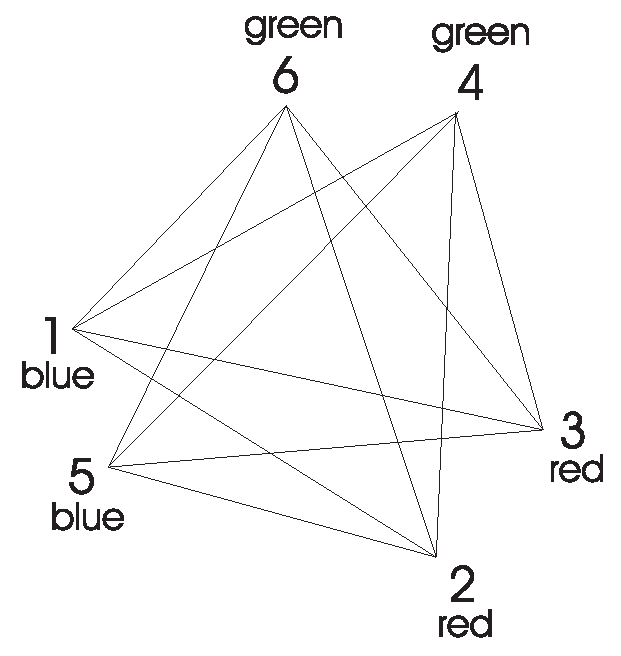
\includegraphics[width=2in,height=2in]{adjgraph}

\solution{ 

\begin{figure}[h]
\begin{center}
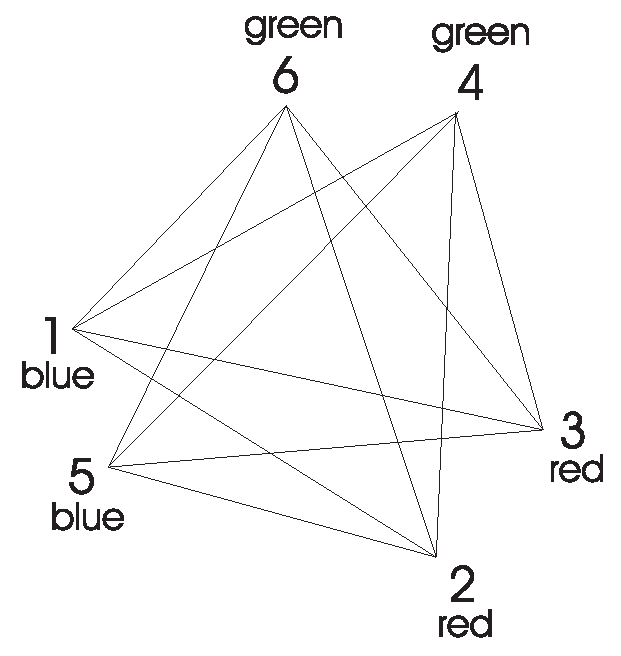
\includegraphics[scale = 0.75 ]{adjgraph}
\end{center}
\end{figure} 

}

\ppart {4} In a graph, we define the \emph{distance} between to vertices to be the length of the shortest path between them. We define the \emph{diameter} of a graph to be the largest distance between any two nodes. What is the diameter of this graph? Explain why.

\solution{This graph has diameter $2$.  There are three pairs of vertices
such that the distance between them is two: $\set{1,5}, \set{2,3}$ and
$\set{4,6}$.  There is an edge between all other pairs of vertices, and
hence the distance between those pairs is $1$.}

\ppart {3} Find a cycle in this graph of maximum length and explain
why it has maximum length.

%\textbf{NICK VERSION: The cycle with edges $\{\edge{1}{6}, \edge{6}{3}, \edge{3}{4}, \edge{4}{5}, \edge{5}{2}, \edge{2}{1} \}$ has length 6.} 
\solution{The cycle 1-6-3-4-5-2-1 has length 6.  Since any cycle can contain each vertex at most once, no cycle can have
 length greater than 6.  Therefore the stated cycle has maximum length.}

\ppart {4} Give a coloring of the vertices that uses the minimum
number of colors. Prove that this a minimum coloring.

\solution{The diagram above shows a 3-coloring.  The chromatic number
 cannot be less than 3, because vertices 1, 2, and 4 are all connected
 and therefore must receive distinct colors.  Consequently, the
 chromatic number of the graph is exactly 3.}

 \eparts

 \end{problem}


\begin{problem}{10}
Let $G$ be a graph.  In this problem we show every vertex of odd degree is connected to at least one other vertex of odd degree in $G$.

\begin{problemparts}

\ppart{6} Let $v$ be an odd degree node. Consider the longest walk starting at $v$ that does not repeat any edges (though it may omit some). Let $w$ be the final node of that walk. Show that $w \neq v$.

\solution{Since $v$ has odd degree, the walk contains at least one edge.
Furthermore, the final vertex of the walk cannot be $v$, since the
edges incident to $v$ would then consist of the first and last edge of
the walk plus two edges for each time that the walk crosses $v$--- an
even total.}

\ppart{4} Show that $w$ must also have odd degree.

\solution{The edges incident to the final vertex of the
walk consist of the final edge of the walk plus two edges for each
time that the walk crosses the final vertex, for an odd total.}


\solution{
An alternative solution to the overall problem (but not to the individual parts) can be obtained from the Handshake lemma.

\begin{proof}
The sum of the degrees of the vertices in any connected component is twice the
number of edges in the component.  So there must be an even number of
odd-degree vertices in any connected component.  In particular, if there
is a vertex of odd degree in the component, there must be an odd number of
additional odd-degree vertices connected to it.
\end{proof}
}

\eparts
\end{problem}

\end{document}
